%!TEX root = ../thesis.tex

\chapter{Experiments and Results}
\label{cha:experimentsandresults}



% Describe the evaluation you did in a way, such that an independent researcher can repeat it. Cover the following questions:
% \begin{itemize}
%  \item \textit{What is the experimental setup and methodology?} Describe the setting of the experiments and give all the parameters in detail which you have used. Give a detailed account of how the experiment was conducted.
%  \item \textit{What are your results?} In this section, a \emph{clear description} of the results is given. If you produced lots of data, include only representative data here and put all results into the appendix.
% \end{itemize}
%%%%%%%%%%%%%%%%%%%%%%%%%%%%%%%%%

\section{Setup}
\subsection{Workstation}

The main developing tool has been a laptop which has been used for a huge variaty of tasks: write code, debug, check papers and documentation, write notes, etc.
In order to train and make prediciton with deep learning models, an intensive computational resources are required.

This is why in addition, access to a GPU cluster has been provided in order to train models using GPUs.
The Computer Vision Lab provide access to BIWI cluster which has been used to store datasets and models and also as a computation resource. The BIWI cluster consists on 70 computational nodes (CPU only) with a total of 556 processors, 8328 cores and 13.3TB of RAM memory.
In addition, there are the GPU nodes which consists in 75 GPUs with 12GB of GPU memory each one.

\subsection{Software}

All the code developement has been done using the Python3 language.
Python is commonly extended in computer vision and deep learning applications because all the available libraries that provides computational frameworks and also because its easiness developing.

The main library used to develop deep learning models has been PyTorch~\cite{paszke2017automatic}. This library provides high-level features for tensor computation and deep neural networks.
This library is a wrapper in Python which under the hood is writen in C allowing fast performance and strong GPU acceleration.
This library is usually used in the research community because its flexibility, fast code prototyping and easily debugging capabilities.

\section{Datasets}

During the development of this thesis, two segmentation datasets have been used: DAVIS and PASCAL.

\subsection{DAVIS Dataset}

The DAVIS Dataset~\cite{Perazzi2016,PontTuset2017} consists on a Densely Annotated Video Segmentation dataset.
It provides a curated densely annotations for object instances in video sequences.
There are two versions of the dataset: DAVIS 2016~\cite{Perazzi2016} and DAVIS 2017~\cite{PontTuset2017}. The 2016 version provides foreground/background annotations while the 2017 provides annotations for multiple objects and instances in the foreground.
During the work done on this thesis, DAVIS 2017 version has been used.
Some examples of the annotations are shown in \figref{davis} and information about the dataset is also given in \tabref{davis}.

\begin{table}[h]
\centering
\begin{tabular}{l|lllll}
  DAVIS 2017                          & train & val  & test-dev & test-challenge & \textbf{Total} \\
	\hline
  Number of sequences                 & 60    & 30   & 30       & 30             & \textbf{50}    \\
  Number of frames                    & 4219  & 2023 & 2037     & 2180           & \textbf{10459} \\
  Mean number of frames per sequence  & 70.3  & 67.4 & 67.9     & 72.7           & \textbf{69.7}  \\
  Number of objects                   & 138   & 59   & 89       & 90             & \textbf{376}   \\
  Mean number of objects per sequence & 2.30  & 1.97 & 2.97     & 3.00           & \textbf{2.51}
\end{tabular}
\caption{Size of the DAVIS 2017 data splits: number of sequences, frames and annotated objects.}
\label{tab:davis}
\end{table}

\begin{figure}[h]
\centering
\begin{subfigure}{.25\textwidth}
  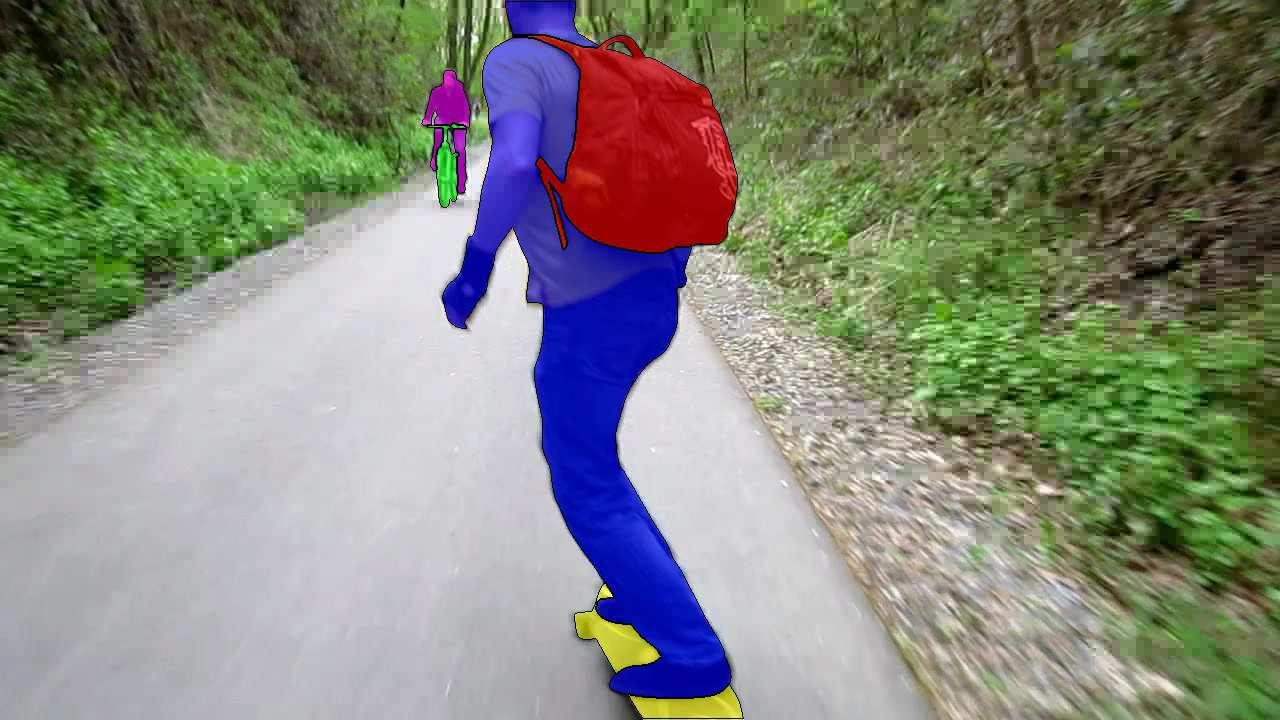
\includegraphics[width=1.\linewidth]{figures/davis_dataset/image_1.jpg}
\end{subfigure}%
\begin{subfigure}{.25\textwidth}
  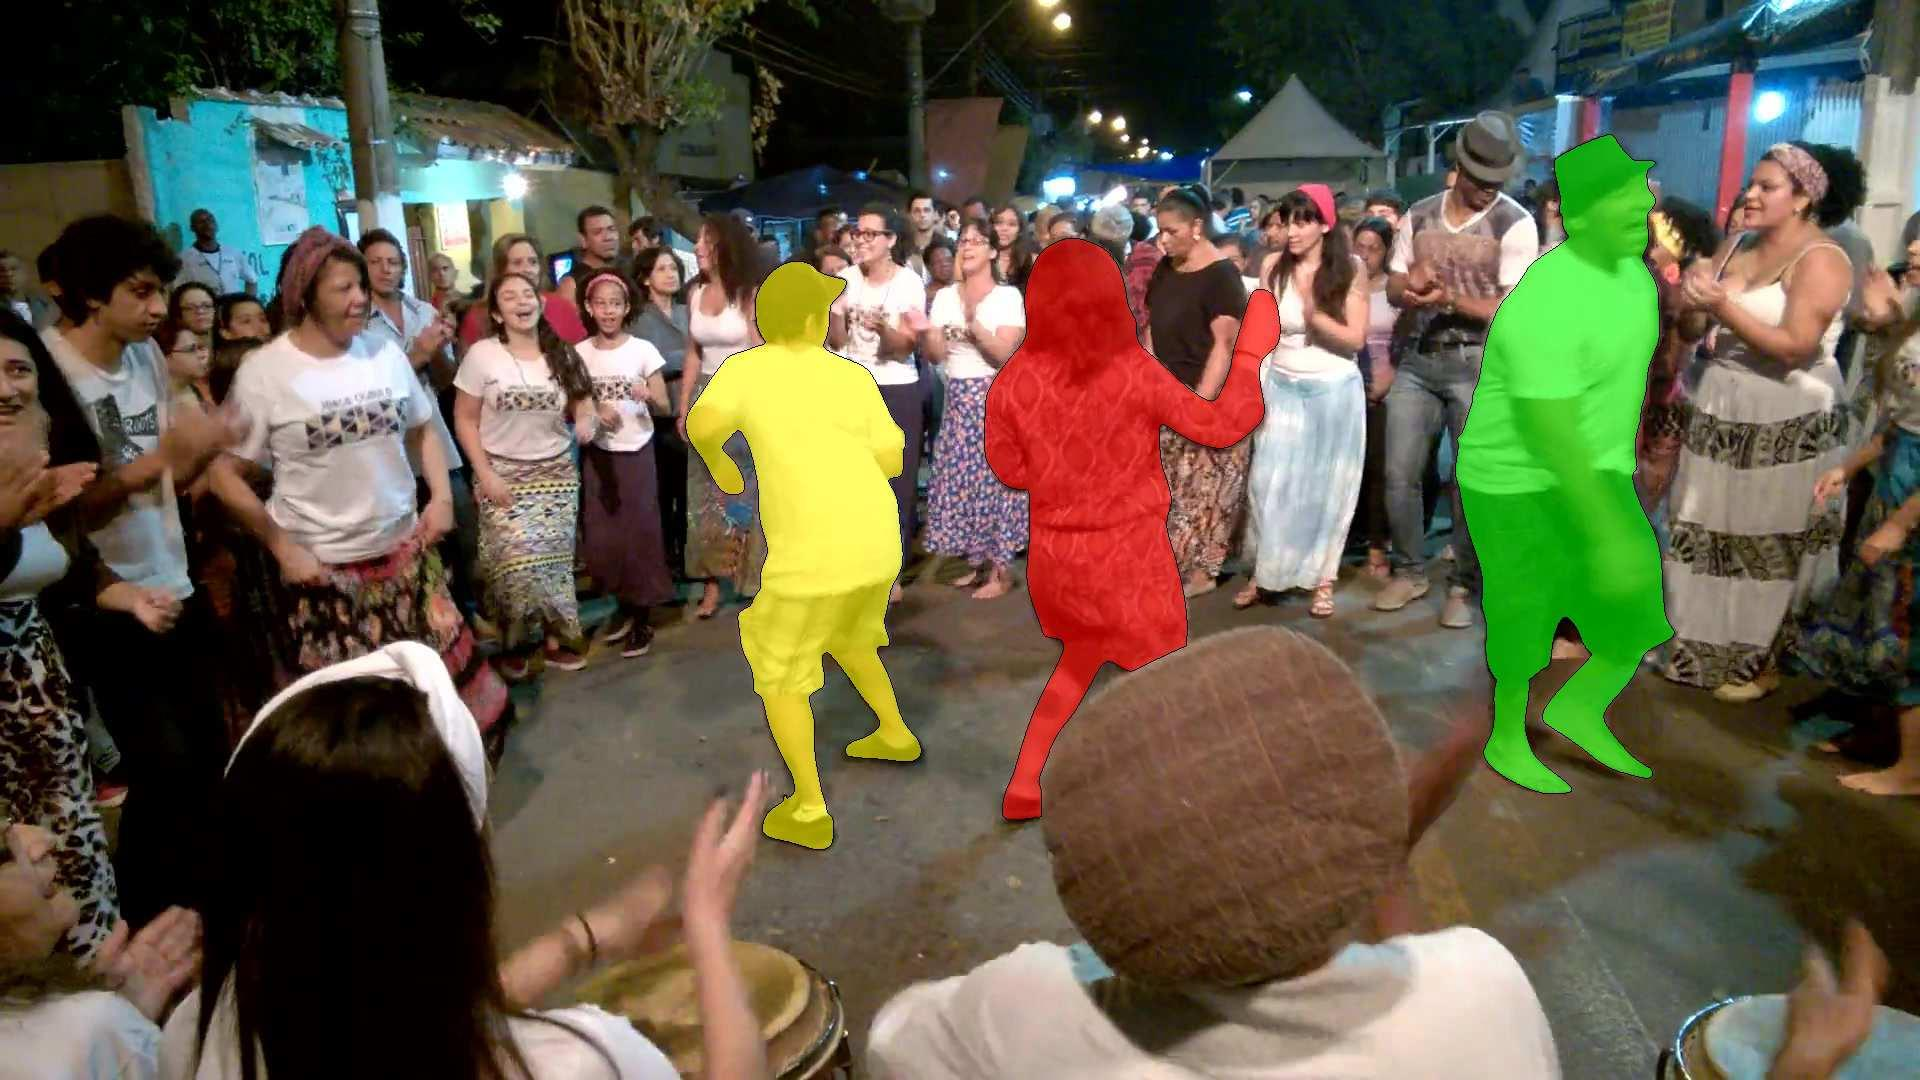
\includegraphics[width=1.\linewidth]{figures/davis_dataset/image_2.jpg}
\end{subfigure}%
\begin{subfigure}{.25\textwidth}
  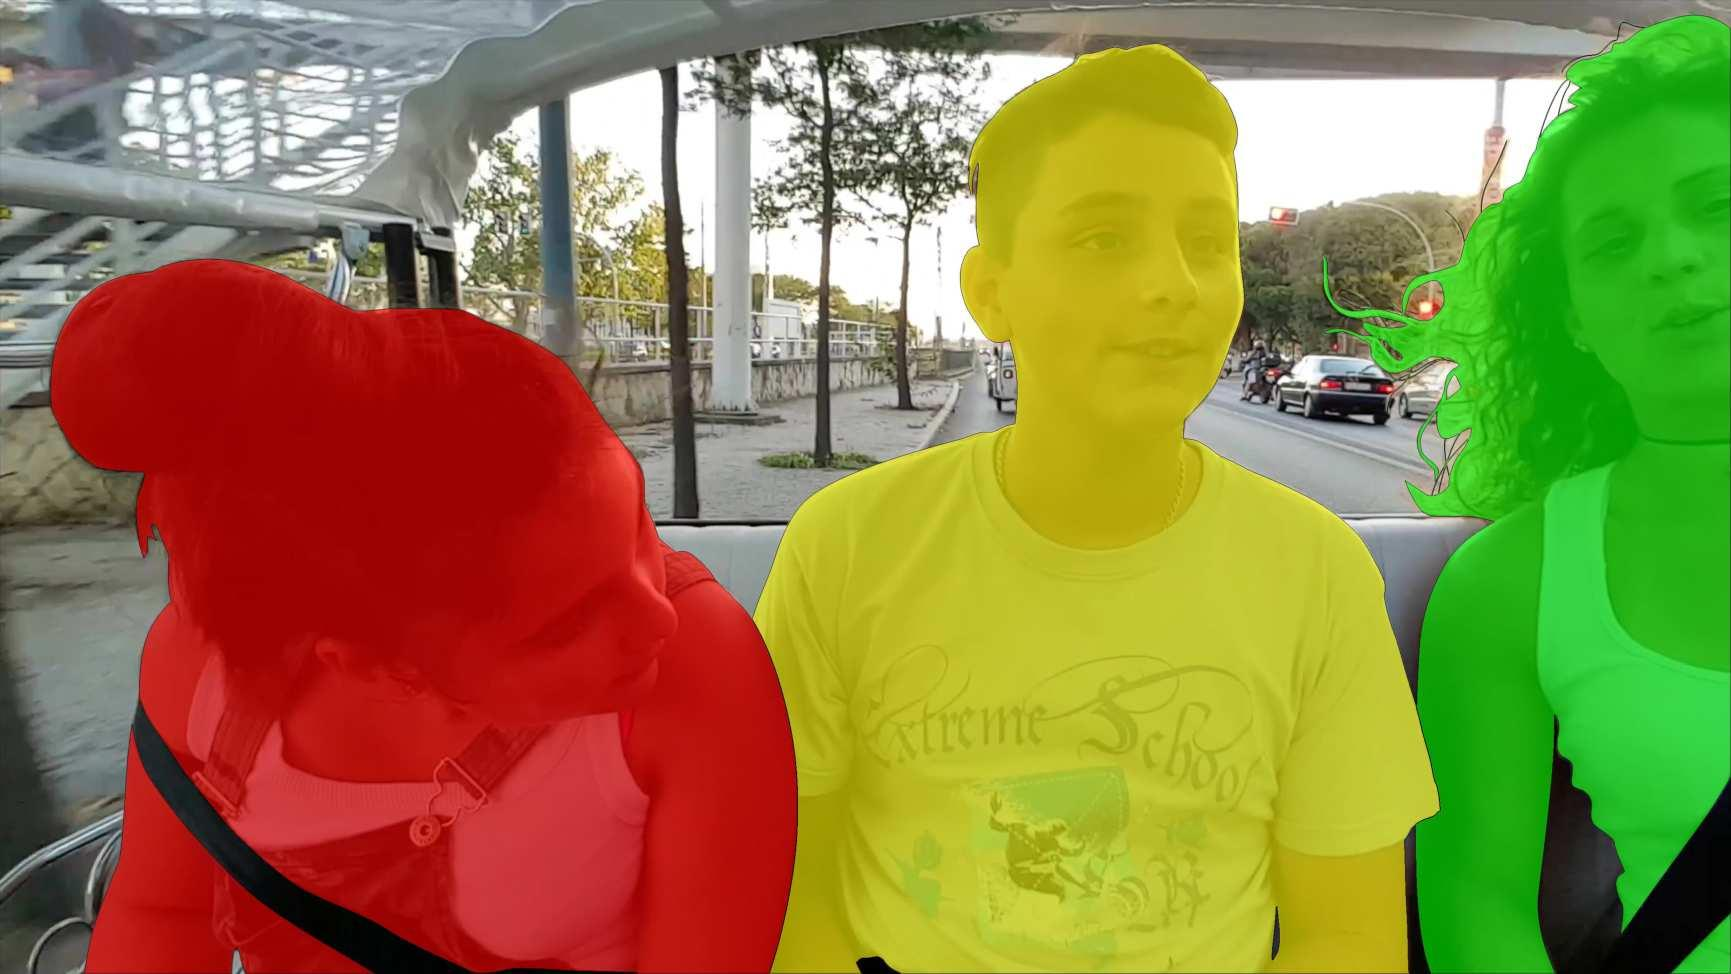
\includegraphics[width=1.\linewidth]{figures/davis_dataset/image_3.jpg}
\end{subfigure}%
\begin{subfigure}{.25\textwidth}
  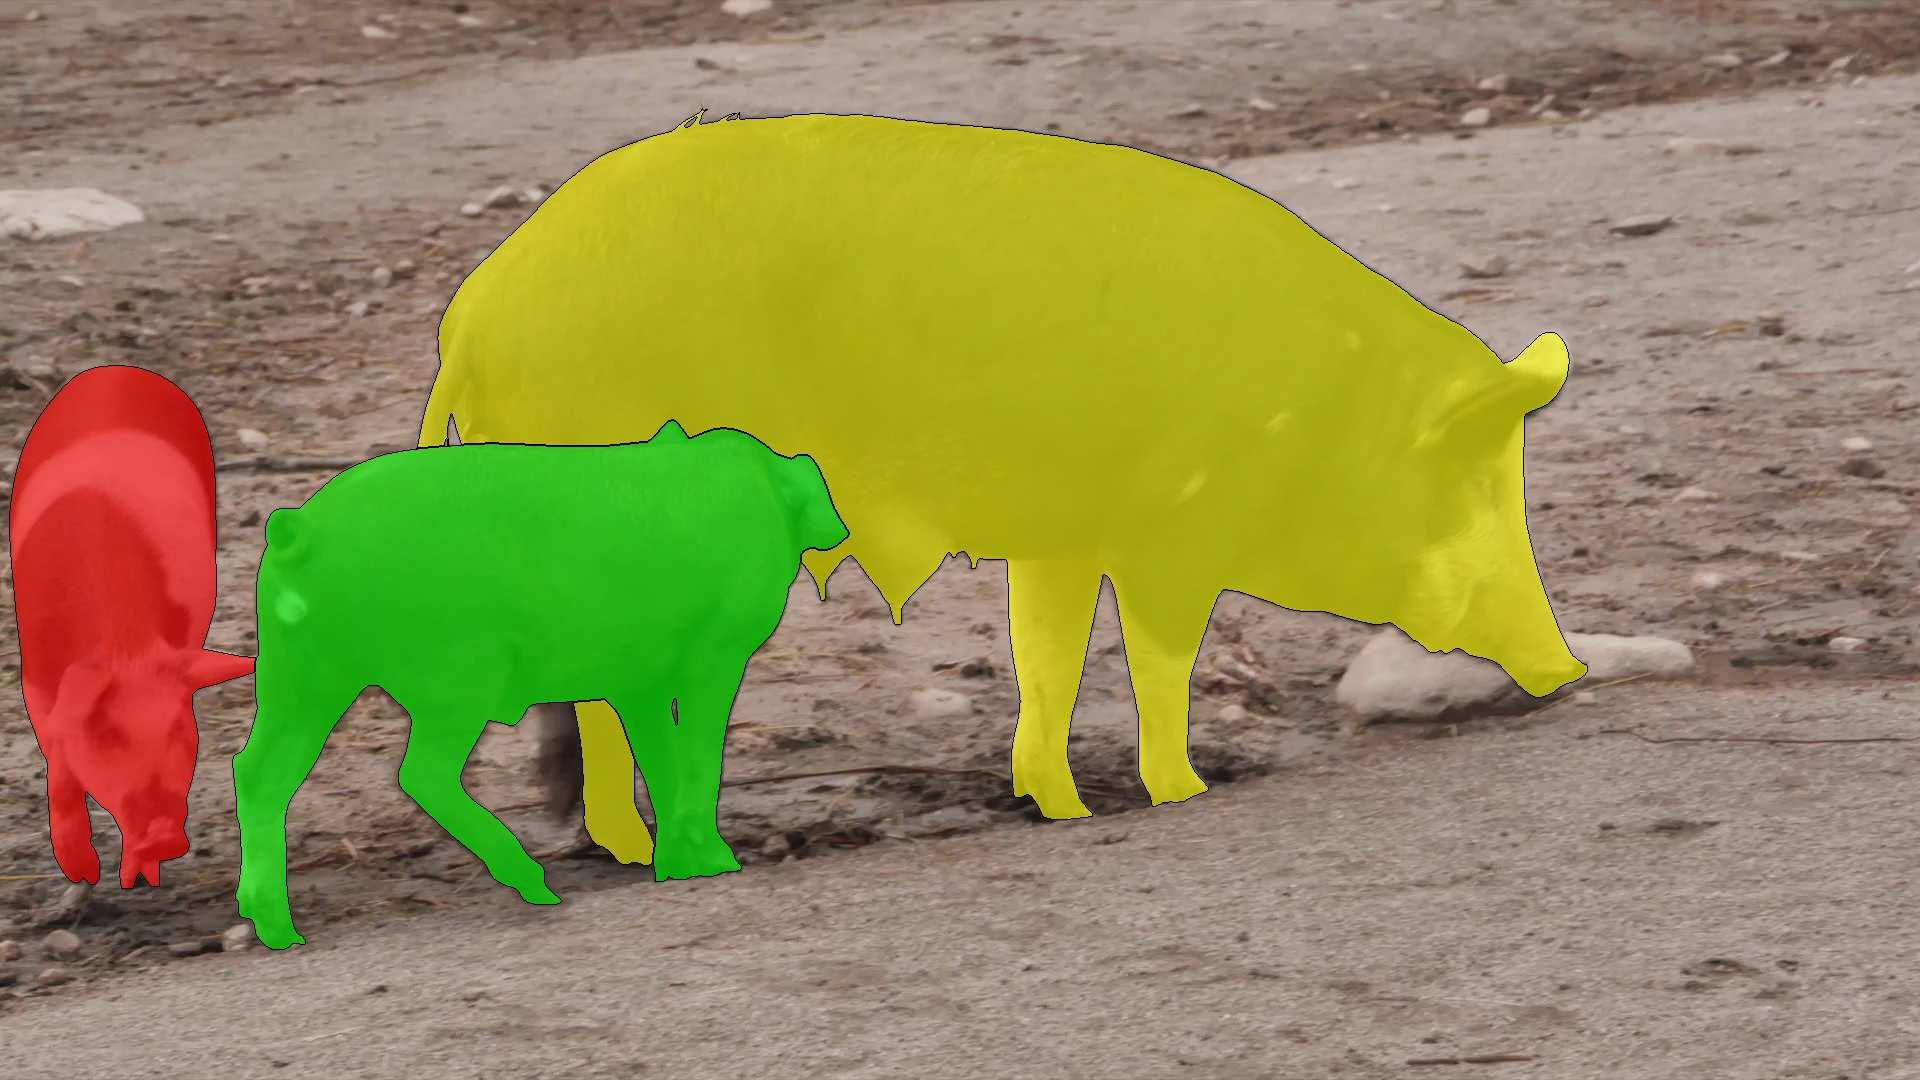
\includegraphics[width=1.\linewidth]{figures/davis_dataset/image_4.jpg}
\end{subfigure}
\caption{Example of annotations on DAVIS 2017 Dataset.}
\label{fig:davis}
\end{figure}


The DAVIS dataset owners also organize a challenge to evaluate the performance of different segmentation method.
This challenge have two branches which are the following:

\paragraph{Semi-supervised}

Consists on generate a prediction given only the ground truth mask of the first frame.
This gives information to the about which is the object intended to be segmented.

\paragraph{Unsupervised}

As the name specifies, no information is given about the object that must be segmented.
To solve this, the segmentation methods rely on the frames to infer the foreground and background.

\subsection{PASCAL Dataset}

PASCAL Dataset~\cite{Everingham10} is a dataset used to benchmark vision object category recognition, detections and segmentation.
Consist on images containing 20 visual object classes and provides multiple annotation for different computer vision tasks: detection and segmentation.
The segmentation annotations consist on masks over instances belonging to the 20 classes, which lead with images with multiple instance annotations.

During this thesis, the segmentation annotations from PASCAL VOC 2012 have been used. The information about the number of instances per split can be found on \tabref{pascal} and some samples of the dataset at \figref{pascal}.

\begin{table}[h]
\centering
\begin{tabular}{l|lll}
PASCAL VOC 2012                    & train & val  & \textbf{Total} \\
\hline
Number of images                   & 1464  & 1449 & \textbf{2913}  \\
Number of instances                & 3507  & 3427 & \textbf{6934}  \\
Mean number of instances per image & 2.40  & 2.37 & \textbf{2.38}  \\
\end{tabular}
\caption{Size of the PASCAL VOC 2012 data splits: number of images and annotated objects.}
\label{tab:pascal}
\end{table}


\begin{figure}[h]
\centering
% Images
\begin{subfigure}{.25\textwidth}
  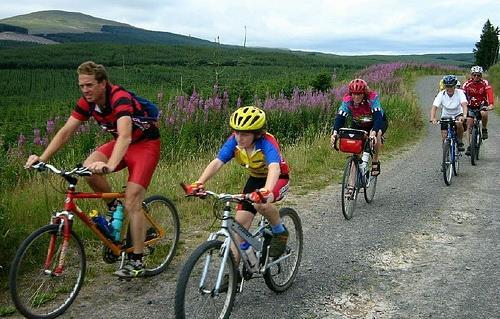
\includegraphics[width=1.\linewidth,height=0.618\linewidth]{figures/pascal_dataset/image-1.jpg}
\end{subfigure}%
\begin{subfigure}{.25\textwidth}
  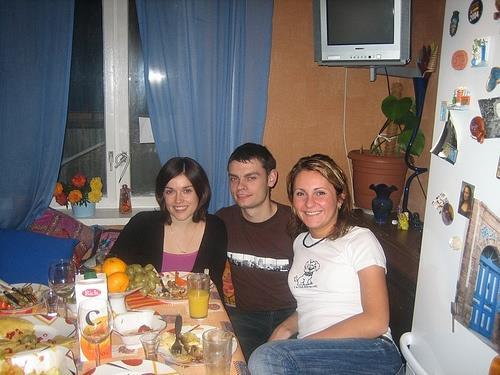
\includegraphics[width=1.\linewidth,height=0.618\linewidth]{figures/pascal_dataset/image-2.jpg}
\end{subfigure}%
\begin{subfigure}{.25\textwidth}
  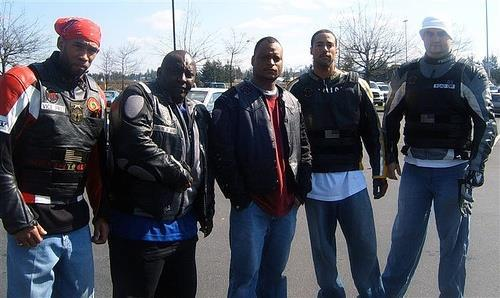
\includegraphics[width=1.\linewidth,height=0.618\linewidth]{figures/pascal_dataset/image-3.jpg}
\end{subfigure}%
\begin{subfigure}{.25\textwidth}
  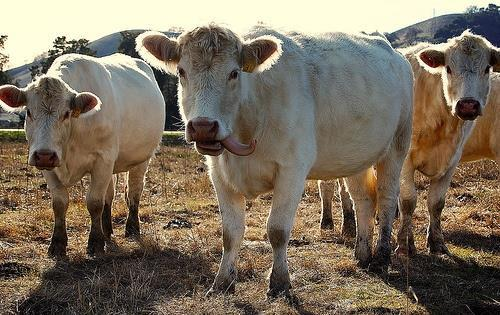
\includegraphics[width=1.\linewidth,height=0.618\linewidth]{figures/pascal_dataset/image-4.jpg}
\end{subfigure}
% Annotations
\begin{subfigure}{.25\textwidth}
  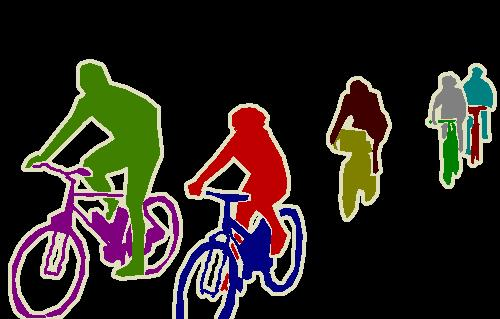
\includegraphics[width=1.\linewidth,height=0.618\linewidth]{figures/pascal_dataset/annotation-1.jpg}
\end{subfigure}%
\begin{subfigure}{.25\textwidth}
  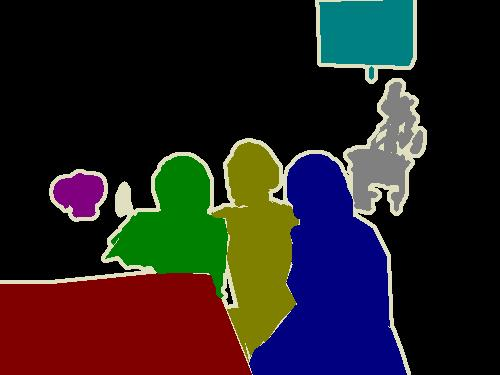
\includegraphics[width=1.\linewidth,height=0.618\linewidth]{figures/pascal_dataset/annotation-2.jpg}
\end{subfigure}%
\begin{subfigure}{.25\textwidth}
  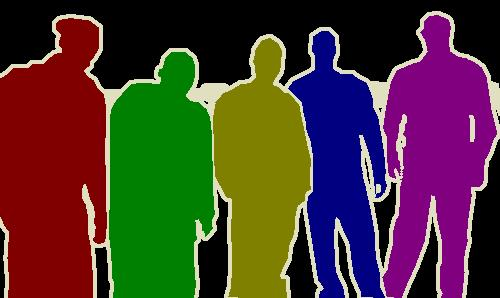
\includegraphics[width=1.\linewidth,height=0.618\linewidth]{figures/pascal_dataset/annotation-3.jpg}
\end{subfigure}%
\begin{subfigure}{.25\textwidth}
  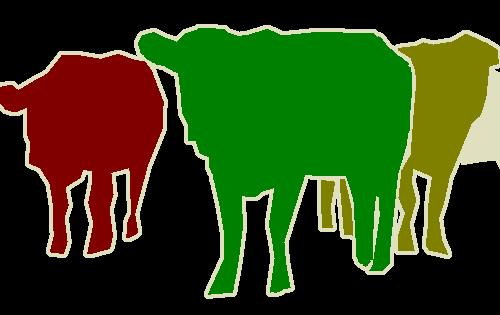
\includegraphics[width=1.\linewidth,height=0.618\linewidth]{figures/pascal_dataset/annotation-4.jpg}
\end{subfigure}
\caption{Example of images (top) and annotations (bottom) on PASCAL VOC 2012 Dataset.}
\label{fig:pascal}
\end{figure}


%%%%%%%%%%%%%%%%%%%%%%%%%%%%%%%%%

\section{Experiments}

\subsection{Tracking}

% List all the experiments and its results regarding the tracking points on DAVIS\@.
% Put mostly the results in the dashboard here.

% Show the results of tracking points using triplet sampling. Improving the coverage.

% Then the results pivoting to instance segmentation. Put here the results of the notebook.

Define metrics Precision pixel distance.

Comment training parameters

Results of tracking point regressing a heatmap for his location. Define Baseline and explain MDNET results.

\begin{figure}[h]
	\centering
	%!TEX root = ../thesis.tex

\begin{tikzpicture}
  \begin{axis}[
      set layers,
      width=\textwidth,
      height=.5\textwidth,
      width=\linewidth, % Scale the plot to \linewidth
      grid=both,
      grid style=dotted,
      minor ytick={0,0.05,...,1.1},
      ytick={0,0.1,...,1.1},
      yticklabels={0,.1,.2,.3,.4,.5,.6,.7,.8,.9,1},
      ymin=0, ymax=1,
      xmin=0, xmax=50,
      xlabel=Distance (pixels), % Set the labels
      ylabel=Detection Rate,
      legend columns=1,
      %transpose legend,
      cycle list name=exotic,
      legend pos= south east,
      legend style={/tikz/every even column/.append style={column sep=3mm}},
      % legend style={at={(0.5,-0.2)},anchor=north},
      % x tick label style={rotate=90,anchor=east}
    ]
    \addplot+[smooth, cyan, mark=none, line width=1]
    table [x=Threshold, y=Baseline, col sep=comma] {data/precission_threshold_curves.csv};
    \addlegendentry{Baseline}

    \addplot+[smooth, red, mark=none, line width=1]
    table [x=Threshold, y=MDNet, col sep=comma] {data/precission_threshold_curves.csv};
    \addlegendentry{MDNet}

    % \addplot+[smooth, green, mark=none, line width=1]
    % table [x=Threshold, y=Hourglass w/o Parent Network 1HG x2 sigma 5, col sep=comma] {data/precission_threshold_curves.csv};
    % \addlegendentry{Hourglass}

    % \addplot+[smooth,  mark=none, line width=1]
    % table [x=Threshold, y=ResNet101 sigma20, col sep=comma] {data/precission_threshold_curves.csv};
    % \addlegendentry{ResNet101}

    \addplot+[smooth,  mark=none, line width=1]
    table [x=Threshold, y=ResNet50 sigma40, col sep=comma] {data/precission_threshold_curves.csv};
    \addlegendentry{ResNet50}

    \addplot+[smooth,  mark=none, line width=1]
    table [x=Threshold, y=ResNet50 Multiscale sigma964824, col sep=comma] {data/precission_threshold_curves.csv};
    \addlegendentry{ResNet50 Multiscale}

  \end{axis}
\end{tikzpicture}

  \label{fig:tracking_point_regression}
	\caption{Precission performance for point regression.}
\end{figure}

In addition to this metric, in order to see if our model has been able to learn the representation of the object to track, we compute the a coverage factor.
This coverage factor is defined as the accuracy of the model to predict a tracked point inside the ground truth mask of the object to track.
These results are showed at \tabref{coverage_tracking_heatmap}.

\begin{table}[h]
  \centering
  \begin{tabular}{l|l}
    \toprule
    Method              & Coverage \\
    \midrule
    Baseline            & 0.428    \\
    MDNET               & 0.851    \\
    Hourglass           & 0.812    \\
    % ResNet101           & 0.912 \\
    ResNet50            & 0.912    \\
    ResNet50 Multiscale & 0.940    \\
    \bottomrule
  \end{tabular}
  \caption{Coverage for different methods that regress the heatmap. }
  \label{tab:coverage_tracking_heatmap}
\end{table}


Then we switched to ResNet101 with the weights pre-trained on VOC.
% Tracking the features vector of the ResNet101 pretrained with VOC\@.
% The best tracking was performed using cosine distance and averaging the representation of $3 \times 3$ patches.
% Backbone architecture ResNet101.

\begin{figure}[h]
  \centering
  %!TEX root = ../thesis.tex

\begin{tikzpicture}
  \begin{axis}[
      set layers,
      width=\textwidth,
      height=.5\textwidth,
      width=\linewidth, % Scale the plot to \linewidth
      grid=both,
      grid style=dotted,
      minor ytick={0,0.05,...,1.1},
      ytick={0,0.1,...,1.1},
      yticklabels={0,.1,.2,.3,.4,.5,.6,.7,.8,.9,1},
      ymin=0, ymax=1,
      xmin=0, xmax=50,
      xlabel=Distance (pixels), % Set the labels
      ylabel=Detection Rate,
      legend columns=1,
      %transpose legend,
      cycle list name=exotic,
      legend pos= north west,
      legend style={/tikz/every even column/.append style={column sep=3mm}},
      % legend style={at={(0.5,-0.2)},anchor=north},
      % x tick label style={rotate=90,anchor=east}
    ]

    % \addplot+[smooth,  mark=none, line width=1]
    %   table [x=Threshold, y=Features Metric Learning Quadplet Loss (480p) Basic metriccosine patchsize3, col sep=comma] {data/precission_threshold_curves.csv};
    % \addlegendentry{Double Triplet Loss D=2048}

    \addplot+[smooth,  mark=none, line width=1]
      table [x=Threshold, y=Features Metric Learning Triplet Loss (480p) D128 Basic metriccosine patchsize3, col sep=comma] {data/precission_threshold_curves.csv};
    \addlegendentry{Triplet Loss D=128}

    \addplot+[smooth,  mark=none, line width=1]
      table [x=Threshold, y=Features Metric Learning (480p) Basic metriccosine patchsize3, col sep=comma] {data/precission_threshold_curves.csv};
    \addlegendentry{Triplet Loss D=2048}

    \addplot+[smooth,  mark=none, line width=1]
    table [x=Threshold, y=Features ResNet Basic metriccosine patchsize3, col sep=comma] {data/precission_threshold_curves.csv};
    \addlegendentry{Pre-Trained VOC D=2048}

    \addplot+[smooth,  mark=none, line width=1]
    table [x=Threshold, y=Baseline, col sep=comma] {data/precission_threshold_curves.csv};
    \addlegendentry{Baseline}

  \end{axis}
\end{tikzpicture}

  \label{fig:tracking_metric_learning}
  \caption{Precission performance for pixel representation tracking.}
\end{figure}

Then check the coverage on \tabref{coverage_tracking_metric_learning}

\begin{table}[h]
  \centering
  \begin{tabular}{l|l}
    \toprule
    Method                       & Coverage \\
    \midrule
    Baseline                     & 0.428    \\
    Pre-Trained VOD $D=2048$     & 0.620    \\
    Triplet Loss $D=2048$        & 0.750    \\
    Triplet Loss $D=128$         & 0.911    \\
    Double Triplet Loss $D=2048$ & 0.885    \\
    \bottomrule
  \end{tabular}
  \caption{Coverage for different tracking methods trained with metric learning. }
  \label{tab:coverage_tracking_metric_learning}
\end{table}


